\chapter{Next Steps}
\label{chap:nextsteps}
\section{Improvements}
\label{sec:nextsteps_improvements}

When creating a tool for other developers, it is important to keep everything as intuitive and simple as possible, while also supporting many different features to allow more flexibility. Decisions about how to implement certain functionality in Utility Designer were based on these criteria. However, because development time was limited, the focus had to be on the most important features, while others were not yet implemented.

If this project continues, here are some recommended features to consider implementing:

\paragraph{More Base Types:}
When creating a new consideration, there is an option to select its type. Currently there is only "float", but considerations should support more types like "int", "bool", etc. Implementing this is not a very quick task, as everything that uses considerations needs to be able to adapt to the specified type. For example, the curve for evaluators would work differently for a consideration of type "bool".

\paragraph{Inheritance:}
The concept of utility AI shines when it comes to creating multiple characters, all with the same set of states, but each with different priorities for each state. An example of this could be a civilisation simulation where each person has slightly different priorities for each action. This is currently possible by copying and pasting the Utility Behaviour, but adding, say, a new state to the world would mean adding that new state to each copied behaviour separately. Thus the idea of inheritance, where all NPCs would inherit from a base behaviour and then only need to adjust their weights according to their preferences. Consequently, any new state addition would only need to be implemented in the base behaviour itself.

\paragraph{Renaming:}
Currently, strings are used to access Consideration Sets and Considerations, representing their names. When renaming them, all occurrences in the code and also in the editor window have to be changed manually. An automatic way to rename them would therefore be useful.

\paragraph{Undo / Redo:}
Utility Designer doesn't support hotkeys to undo or redo actions. The cleanest way to implement this would probably be to use a SerializedObject, which would involve a lot of code refactoring.

\paragraph{Blackboard:}
In the context of a behaviour tree, a blackboard is a place where globally accessible data is stored and can be used by different nodes in the tree. It's essentially a data store that holds variables and information that different nodes within the behaviour tree can use to perform their tasks or make decisions. Utility Designer does not currently implement a blackboard, but it would be a nice feature to have, but it is not necessary for the core functionality of a behaviour tree.

\paragraph{Backwards Compatibility:}
The tool was created in Unity 2022, as the UI toolkit in this version is more stable than in previous versions. It is currently only compatible with the 2022 version, and making it compatible with earlier versions would make it available to a wider range of developers.

\section{Publishing To The Unity Asset Store}
\label{sec:nextsteps_publishtounityassetstore}

At the time of writing, the Utility Designer has been submitted to the Asset Store, but is still awaiting review by Unity. It has started at a queue position of \#2650, which means it will take about 30 working days for it to be reviewed. Once the asset has been reviewed and accepted, it will be available in the Unity Asset Store. It is possible that the asset will be rejected. In this case, further changes to the asset will be required before it can be resubmitted, depending on the reasons for the rejection.

The tool has been submitted as a free assets to increase the chances of getting more feedback from the community. This feedback can then be used to make improvements and to follow up with updates according to the feedback received or other changes as described in the previous section. The preview of the store page looks as follows:

\begin{figure}[H]
    \centering
    \begin{minipage}{0.49\textwidth}
        \centering
        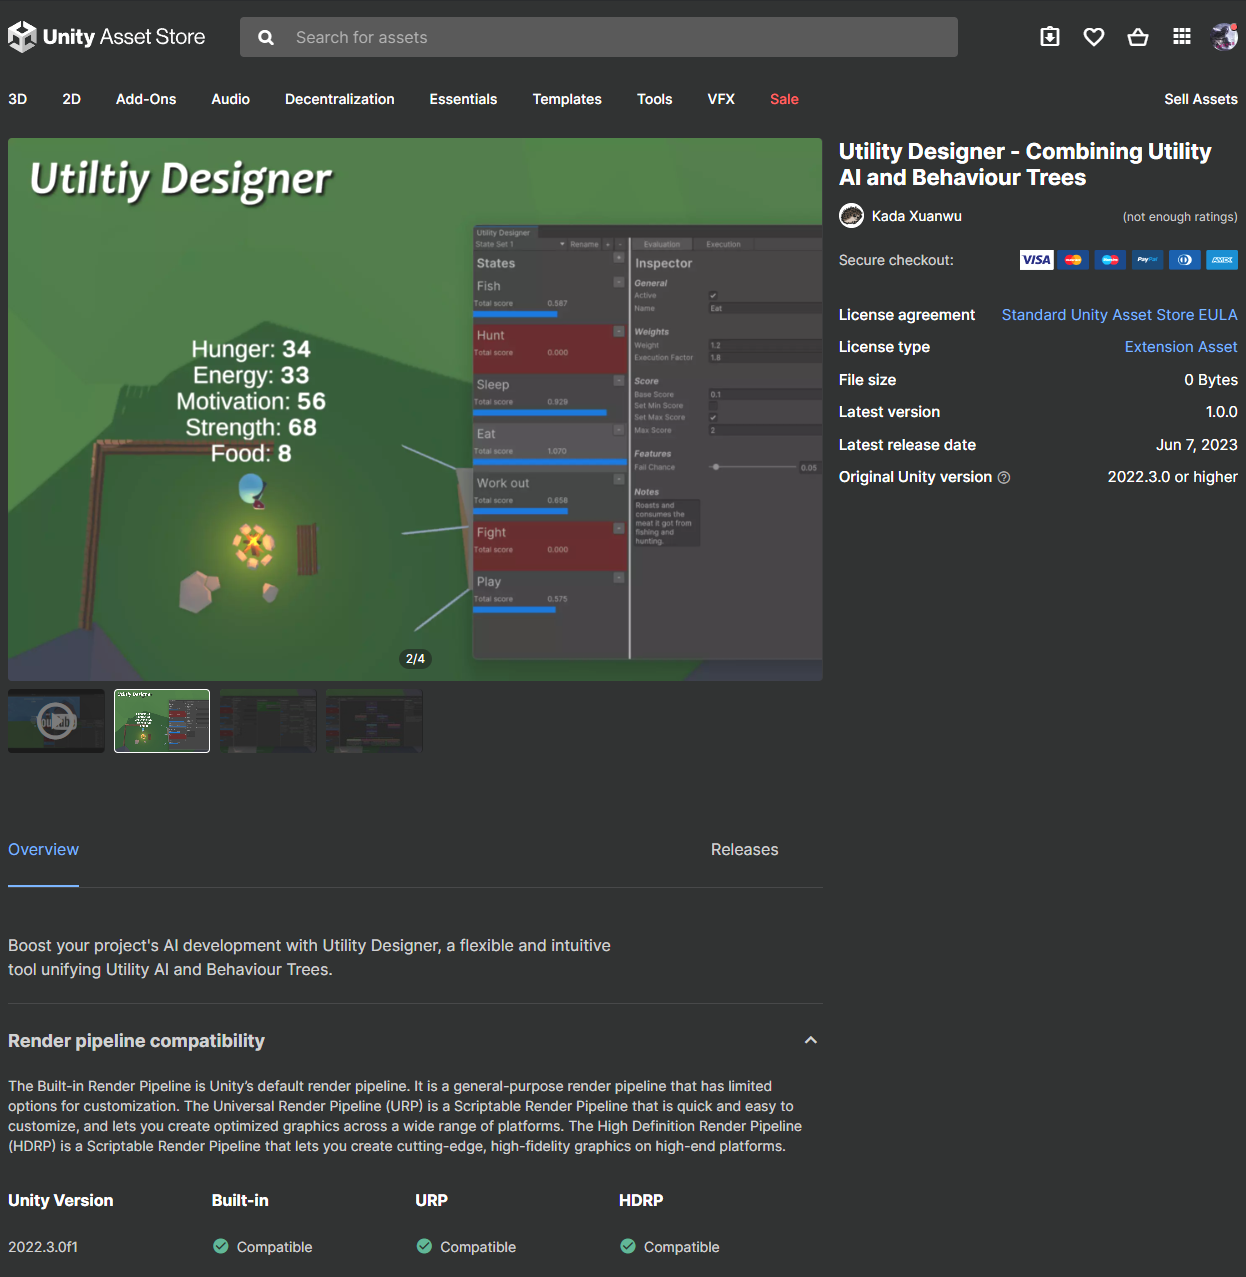
\includegraphics[scale=0.26]{images/asset_store_page_1.png}
        \caption{Asset Store Page Preview 1}
        \label{fig:asset_store_page_1}
    \end{minipage}\hfill
    \begin{minipage}{0.49\textwidth}
        \centering
        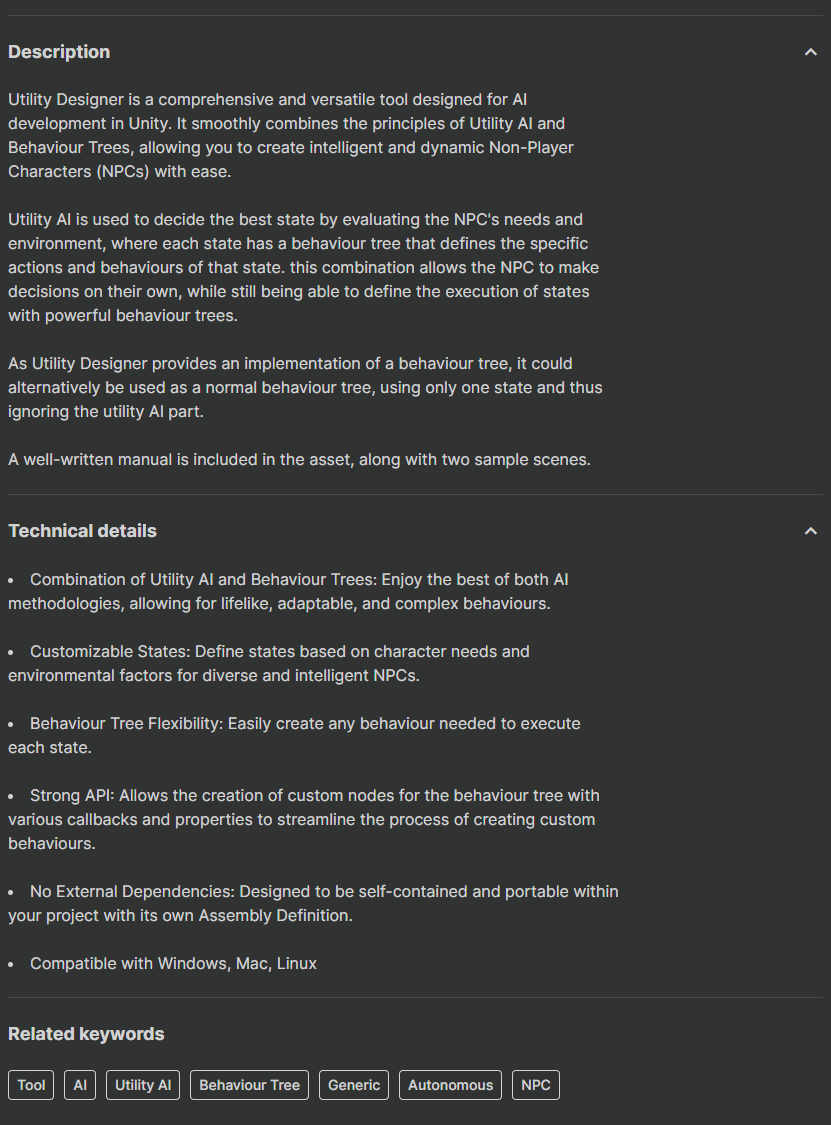
\includegraphics[scale=0.26]{images/asset_store_page_2.png}
        \caption{Page Preview 2}
        \label{fig:asset_store_page_2}
    \end{minipage}
\end{figure}

\newpage

There are several steps involved in preparing and publishing an asset, from asset preparation to submission and approval.

\paragraph{Preparing The Asset}

\begin{enumerate}
    \item \textbf{Asset Development:} The asset must be fully developed and working correctly, following Unity's best practices for asset development.
    \item \textbf{Documentation:} Comprehensive documentation should be provided for the asset. This should include clear instructions on how to use the asset and any known issues.
    \item \textbf{Testing:} The asset should be thoroughly tested to ensure that it works as expected.
\end{enumerate}

\paragraph{Packaging The Asset}

\begin{enumerate}
    \item \textbf{Organizing Files:} All files should be neatly organised in a clear folder structure. It is advisable to include an example folder containing at least one example scene and a documentation file.
    \item \textbf{Package Setup:} Unity provides an 'Export Package' option under the 'Assets' menu. This can be used to create a Unity package file (.unitypackage) of the asset.
\end{enumerate}

\paragraph{Submitting The Asset}

\begin{enumerate}
    \item \textbf{Creating A Publisher Account:} A Unity Publisher account is required to submit assets to the Unity Asset Store. The instructions on the Unity Asset Store can be followed to set up the account.
    \item \textbf{Asset Submission:} Once the Publisher account has been set up, the asset can be submitted for approval. This submission includes the necessary information such as the asset name, description, category, price and package file.
    \item \textbf{Images And Media:} High quality images and video should be provided to showcase the asset. This visual content is critical to marketing the asset to potential users.
    \item \textbf{Approval Wait Time:} The Unity team will review each submission. If approved, the asset becomes available for purchase in the Unity Asset Store. If not approved, Unity will provide feedback on what needs to be addressed. How long this process takes depends on the number of submissions they receive.
\end{enumerate}

\paragraph{After Approval}

\begin{enumerate}
    \item \textbf{Customer Support:} It is important to be prepared to provide support to customers. This support can include answering questions about the asset, providing updates and fixing bugs.
    \item \textbf{Updates And Maintenance:} Keeping the asset updated to ensure compatibility with the latest versions of Unity is critical. Addressing bugs promptly and incorporating user feedback into future updates is also essential.
\end{enumerate}
